\subsection{Projection Matrix}
\label{Sec:Projection}

Eine Projektionsmatrix wird meistens verwendet um ein dreidimensionales Koordinatensystem auf eine Ebene zu projizieren, sie kann aber auch dafür verwendet werden um ein dreidimensionales Koordinatensystem in ein anderes dreidimensionales Koordinatensystem zu projizieren, was hier Anwendung findet. OpenGL arbeitet mit einem orthografischen Koordinatensystem, ein Koordinatensystem bei dem alle Achsen orthogonal zueinander sind. Alle Achsen haben Werte von -1 bis 1. Wenn man ein anderes Koordinatensystem verwenden will benötigt man eine Projektionsmatrix. Diese projiziert das gewünschte Koordinatensystem in das von OpenGL verwendete. Dabei unterscheidet man zwischen zwei Arten von Projektionsmatrizen: orthografische und perspektivische. Diese projizieren das jeweilige Koordinatensystem in das OpenGL-Koordinatensystem (siehe \cref{img:projection}).

Eine orthografische Projektionsmatrix ist nur eine Skalierungsmatrix, da der Raum in jede Achse nur so gestreckt oder gestaucht werden muss, dass die Begrenzungen -1 und 1 ergeben. Dabei wird der gesamte Raum nicht verformt. Daher ist die Berechnung dieser Matrix auch sehr einfach. Für ein Koordinatensystem mit den Begrenzungen l \& r (links \& rechts) an der X-Achse, t \& b (top \& bottom) an der Y-Achse und n \& f (near \& far) an der Z-Achse:
$$ M_{o} = \begin{pmatrix}
\dfrac{2}{r-l} & 0 & 0 & \dfrac{r+l}{l-r} \\
0 & \dfrac{2}{t-b} & 0 & \dfrac{t+b}{b-t} \\
0 & 0 & \dfrac{2}{n-f} & \dfrac{f+n}{n-f} \\
0 & 0 & 0 & 1
\end{pmatrix} $$

Eine perspektivische Projektionsmatrix projiziert eine perspektivisches Koordinatensystem in das OpenGL-Koordinatensystem. In einem perspektivischen Koordinatensystem verlaufen in einer Achsenrichtung alle parallele Geraden in diese Richtung zu genau einem Punkt, dem Fluchtpunkt. Ein bekanntes Beispiel dafür sind Schienen, die so aussehen als würden sie am Horizont zusammenlaufen. So nehmen wir die Welt war. Idealer weise wäre dieser Punkt unendlich weit weg. Da so eine Berechnung im Programm nicht möglich ist, wird der Raum in die Ferne durch die \textit{far plane} begrenzt.
Für ein Koordinatensystem mit den Begrenzungen l \& r (links \& rechts) an der X-Achse, t \& b (top \& bottom) an der Y-Achse und n \& f (near \& far) an der Z-Achse:

$$ M_{p} = \begin{pmatrix}
\dfrac{2n}{r-l} & 0 & \dfrac{r+l}{r-l} & 0 \\
0 & \dfrac{2n}{t-b} & \dfrac{t+b}{t-b} & 0 \\
0 & 0 & \dfrac{-(f+n)}{f-n} & \dfrac{-2fn}{f-n} \\
0 & 0 & -1 & 0
\end{pmatrix} $$
(vgl. Songho's Webseite \cite{ProjectionMatrixWeb})

Der Unterschied zwischen dem near und far Wert sollte möglichst gering sein, da sonst Präzisionsprobleme im Depth-Buffer auftreten können, da dieser eine höhere Präzision in der Nähe der Kamera besitzt und zusätzlich mit Fließkommazahlen arbeitet, welche ebenfalls noch einmal eine höhere Präzision gegen 0 haben. Die Wahl dieser Werte ist dem User der Engine überlassen, aber es sollte immer der kleinste akzeptierbare Wert für die Szene sein. (vgl. Khronos Website \cite{DepthProblem})

\begin{figure}[h]
	\centering
	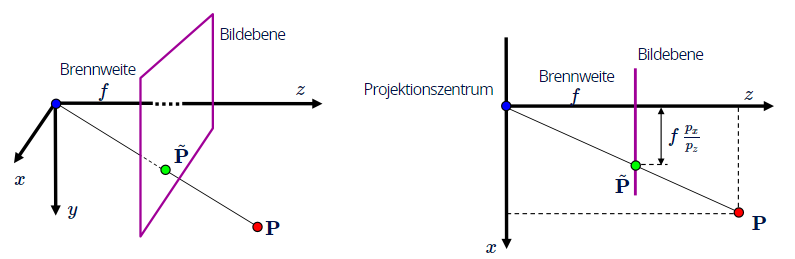
\includegraphics[width=\textwidth]{02theorie/perspektivischeprojektion.png}
	Quelle: \url{http://www.songho.ca/opengl/gl_projectionmatrix.html}	
	14.01.2017
	\caption{Projektions Koordinatensysteme}\label{img:projection}
\end{figure}
